\documentclass[11pt]{article}
\usepackage[pdftex]{graphicx}
%Set margins
\setlength{\textheight}{8in}
\setlength{\oddsidemargin}{.125in}
\setlength{\textwidth}{6.25in}

\usepackage{eso-pic}
\newcommand\BackgroundPic{%
\put(0,0){%
\parbox[b][\paperheight]{\paperwidth}{%
\vfill
\centering

\includegraphics[width=\textwidth,height=\textheight,%
keepaspectratio]{logo.png}%
\vfill
}}}

\mdseries 
\begin{document}
\AddToShipoutPicture*{\BackgroundPic}
\title{BrainGrid\\Documentation}
\author{Kawasaki, Fumitaka \and Stiber, Michael}
\date{} %Doesn't show the date

\maketitle

\pagebreak
\tableofcontents
\pagebreak

%-------------------------------------Abstract Section
\section{Abstract} \mdseries 
BrainGrid is an open-source neural-network simulator that is intended to aid scientists and researchers by providing prebuilt code that can be easily modified to fit different models. The program also offers the ability to easily transition to a GPU-centered with little additional work, and providing a potential speedup of up to a twentieth of the original runtime.

\begin{center}
	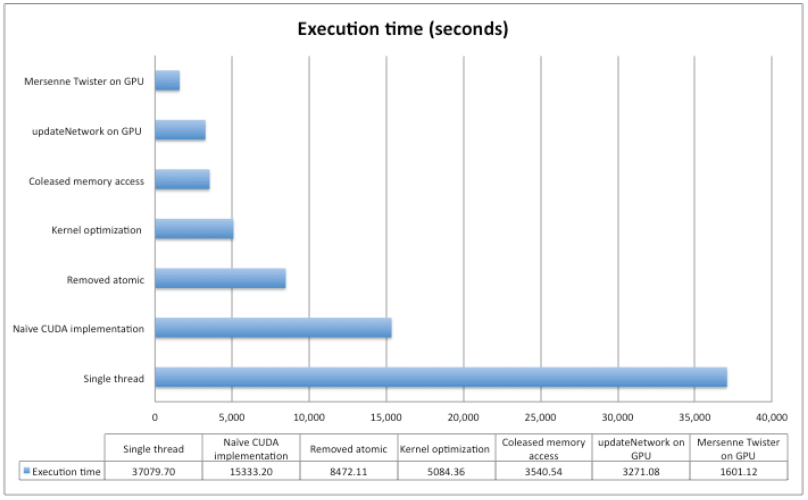
\includegraphics[width=\textwidth]{SpeedComparison.PNG}
\end{center}

\noindent \mdseries The project began as an attempt to reduce the runtime of a simulation of a Leaky Integrate-and-Fire with more than a thousand neurons from two-thousand hours to a much more manageable runtime. Therefore, the program by default comes with a Leaky Integrate-and-Fire simulation preprogrammed. 
\pagebreak

%------------------------------------Design Section
\section{Design} \mdseries 
BrainGrid has undergone recent refactoring and data reorganization due to a need to simplify the implementations of other models. The original legacy code was formatted in an object-oriented fashion, with the multiple simulator/network objects branching out into a complicated list of files and methods that made implementing additional incredibly complex, as implementing said model would require modifying half-a-dozen files and much of these changes would end up being redundant. 
\begin{figure}
	\centering
		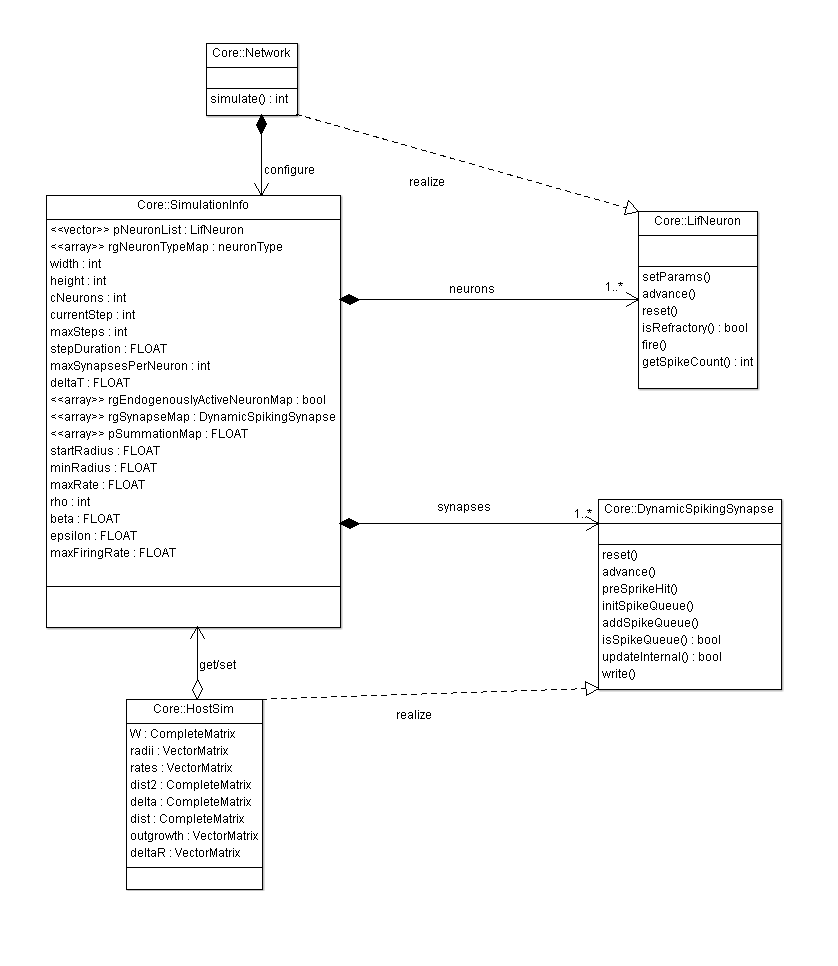
\includegraphics[width=.6\textwidth]{OldDiagram.png}
		\caption{BrainGrid's old design}
\end{figure}
\pagebreak

\noindent \mdseries The refactoring process of BrainGrid reorganized the data structures of the legacy code in order to implement a simpler program structure that prioritizes separating the model-dependent code from the model independent. The new code also stripped away some of the object-oriented structure of the neurons and the synapses, and instead now uses a data-centric structure, which utilizes two different structs as the containers of all neuron and synapse data. This structure was originally designed for the GPU implementation of the simulator, and this refactored version of the simulator simply uses that design for all other implementations as well. This is to simplify transitioning from single-threaded to multi-threaded.

\begin{figure}
	\centering
		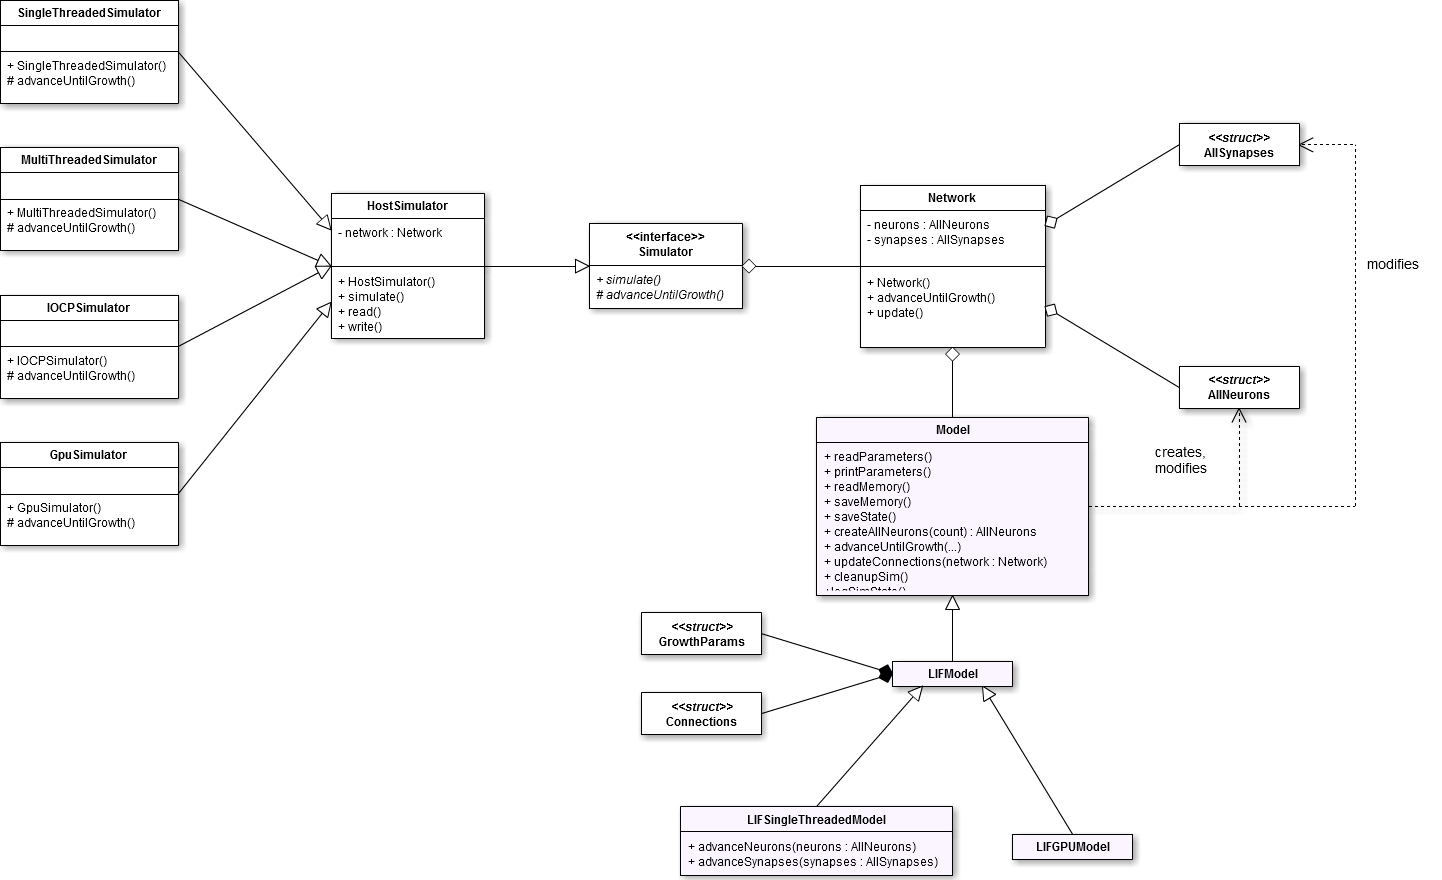
\includegraphics[width=\textwidth]{NewDiagram.png}
		\caption{BrainGrid's new design}
\end{figure}
\pagebreak

%------------------------------------Features Section
\mdseries 
\section{Features}
\begin{itemize}
	\item Multiple simulation architectures:
	\begin{itemize}
		\item	Single-threaded
		\item Multi-threaded
		\item GPU (CUDA)
		\item GPU (AMP)
		\item GPU (OpenMP) --not yet implemented--
		\item GPU (IOCP) --not yet implemented--
		\item GPU (OpenCL) --not yet implemented--
	\end{itemize}
	\item Supported operating systems:
	\begin{itemize}
		\item Microsoft Windows
		\item Linux Distributions
	\end{itemize}
	\item Tools
	\begin{itemize}
		\item GitHub
		\item MATLAB
	\end{itemize}
\end{itemize}
\pagebreak

%------------------------------------User Guide Section
\section{User Guide}
\subsection{Linux Distributions}
\mdseries Upon downloading and extracting the contents of the project, the following steps should be followed to run the simulation.
\begin{enumerate}
	\item	In a terminal window, navigate to the main project folder. 
	\item Run the \verb|make growth| command, which will compile the entire project.
	\item Upon completion, run the command \verb|./growth -t <input file>| where \verb|<input file>| is the full address of the configuration file, examples of which were in the \verb|config| folder.
	\item The program will then run and display the current step and epoc of the simulation. The output of the simulation (after the end of the simulation) will be saved in the \verb|output| folder. 
\end{enumerate}
\subsubsection{Advanced Use}
\mdseries Use of the UNIX command \verb|screen| is recommended in order to allow the process to run in the background. As the simulation is running, the \verb |Ctrl+A and D| keys will detach the . The simulation will continue running in the background, while recording the output of the simulation to the seperate screen. To resume viewing the seperate screen, use the command \verb|screen -r|.

\noindent \mdseries For advanced users, the GCC compiler offers multiple optimization options that may provide some additional speed boost for the CPU-side simulation. It is recommended that, for each level of optimization, the output be verified against unoptimized/less optimized output. The BrainGrid team \bfseries DOES NOT \mdseries recommend using any optimization levels above -02. This level of optimization seems to be unstable, and does not seem to maintain consistent output results.   

\subsection{Microsoft Windows}
TODO
\pagebreak

%------------------------------------Implementing Other Models Section
\section{Implementing Other Models}
TODO
\pagebreak

%------------------------------------Tools Section
\section{Tools}
\subsection{GitHub}
\mdseries GitHub is a source-control system oriented towards the open source community. It offers multiple different features that are advantageous for the project, the most important of which the ability to manage multiple separate versions of the project’s code. This allows the project’s developers the ability to tackle multiple different features and/or bugs.

\noindent \mdseries In order to use GitHub, several tools have been released. The Microsoft Windows, Apple Macintosh software are available on their website.  On Linux distributions, the console is used to manipulate code. As such, the following are instructions on how to install and use GitHub on Linux distributions, focusing on the Ubuntu variety. These instructions assume that the user has already registered with GitHub.

\noindent \mdseries First, the operating system must be updated, and then use apt-get to install GitHub:

\begin{verbatim}
sudo apt-get update
sudo apt-get install git
\end{verbatim}

\noindent \mdseries Next, the username and email settings must be configured properly. 
\begin{verbatim}
git config --global user.name <USERNAME HERE>
git config --global user.email <EMAIL HERE>
\end{verbatim}

\noindent This is when the source code needs to be downloaded from the remote repository. Navigate to the folder where the source code is to be held:
\begin{verbatim}
git clone git://github.com/UWB-Biocomputing/BrainGrid.git
\end{verbatim}

\noindent \mdseries Once the source code is downloaded, the BrainGrid subfolder will be where all the code modifications will occur. Navigate to this subfolder, and use:
\begin{verbatim}
git branch -r
\end{verbatim}

\noindent \mdseries To view the multiple available remote branches (different variations of the code that exist outside the local computer). The GitHub webpage will contain more information about each branch, and how the source code varies in between them. In order to checkout a remote branch, use:
\begin{verbatim}
git branch <LOCAL NAME> origin/<REMOTE BRANCH NAME>
\end{verbatim}

\noindent \mdseries Where <LOCAL NAME> is the name that will represent the local copy of the code. Once this is done, switching in between different local branches can be done by using:
\begin{verbatim}
git checkout <LOCAL NAME> 
\end{verbatim}

\noindent \mdseries To update a local branch with code on the remote version of the branch, use:
\begin{verbatim}
git pull
\end{verbatim}

\noindent \mdseries To save the modifications to the local branch, use:
\begin{verbatim}
git commit -a -m "`<MESSAGE HERE>"'
\end{verbatim}

\noindent \mdseries To move those changes to the remote branch, use:
\begin{verbatim}
git push
\end{verbatim}

\noindent \mdseries Note that Git will prompt the user for additional information.

\subsection{Matlab}
\mdseries For users with MathWork's MATLAB, a subfolder is included with the some sample files that correctly parse BrainGrid's output for use in MATLAB. The project currently only supports output generation during the end of the simulation, but pseudo real-time output may be implemented in the future.
\pagebreak

\section{F.A.Q.}
\bfseries What version of CUDA does the project currently support?

\noindent \mdseries TODO

\noindent \bfseries 

\pagebreak
\section{Acknowledgements}
\mdseries The BrainGrid project has been designed, coded and refactored by multiple individuals over the years. The project has only moved forward thanks to these individuals, who have participated in this team as a labor of love. Those involved include, but are not limited to, the following list:
\begin{itemize}
	\item	Michael Stiber
	\item Fumitaka Kawasaki
	\item Paul Bunn
	\item Chris Burgess
	\item Derek McLean
	\item Hugo Ribeiro
\end{itemize}

\end{document}
